\documentclass[hyperref, a4paper]{ctexart}
\usepackage{lmodern}
\usepackage{amssymb,amsmath}
\usepackage{ifxetex,ifluatex}
\usepackage{fixltx2e} % provides \textsubscript
\ifnum 0\ifxetex 1\fi\ifluatex 1\fi=0 % if pdftex
  \usepackage[T1]{fontenc}
  \usepackage[utf8]{inputenc}
\else % if luatex or xelatex
  \ifxetex
    \usepackage{xltxtra,xunicode}
  \else
    \usepackage{fontspec}
  \fi
  \defaultfontfeatures{Mapping=tex-text,Scale=MatchLowercase}
  \newcommand{\euro}{€}
\fi
% use upquote if available, for straight quotes in verbatim environments
\IfFileExists{upquote.sty}{\usepackage{upquote}}{}
% use microtype if available
\IfFileExists{microtype.sty}{%
\usepackage{microtype}
\UseMicrotypeSet[protrusion]{basicmath} % disable protrusion for tt fonts
}{}
\ifxetex
  \usepackage[setpagesize=false, % page size defined by xetex
              unicode=false, % unicode breaks when used with xetex
              xetex]{hyperref}
\else
  \usepackage[unicode=true]{hyperref}
\fi
\usepackage[usenames,dvipsnames]{color}
\hypersetup{breaklinks=true,
            bookmarks=true,
            pdfauthor={Tian, Jiahe; Hu, Xiaoxiao; Huang, Jiani; Liu, Jiaxing; Shi, Ruixin; Wu, Chenning; Zhang, Cenyuan; Zhang, Yihan; Wang, Chen},
            pdftitle={ 黑盒测试设计与执行},
            colorlinks=true,
            citecolor=blue,
            urlcolor=blue,
            linkcolor=magenta,
            pdfborder={0 0 0}}
\urlstyle{same}  % don't use monospace font for urls
\setlength{\emergencystretch}{3em}  % prevent overfull lines
\providecommand{\tightlist}{%
  \setlength{\itemsep}{0pt}\setlength{\parskip}{0pt}}
\setcounter{secnumdepth}{5}

\title{\vspace{2in} 黑盒测试设计与执行\\\vspace{0.5em}{\large 软件质量保障与测试课程Lab5课程作业(第9组)}}
\author{Tian, Jiahe\footnote{Equal Contribution, Fudan University, 17307130313
  (\href{mailto:tianjh17@fudan.edu.cn}{\nolinkurl{tianjh17@fudan.edu.cn}})} \and Hu, Xiaoxiao\footnote{Equal Contribution, Fudan University, 17302010077
  (\href{mailto:xxhu17@fudan.edu.cn}{\nolinkurl{xxhu17@fudan.edu.cn}})} \and Huang, Jiani\footnote{Equal Contribution, Fudan University, 17302010063
  (\href{mailto:huangjn17@fudan.edu.cn}{\nolinkurl{huangjn17@fudan.edu.cn}})} \and Liu, Jiaxing\footnote{Equal Contribution, Fudan University, 17302010049
  (\href{mailto:jiaxingliu17@fudan.edu.cn}{\nolinkurl{jiaxingliu17@fudan.edu.cn}})} \and Shi, Ruixin\footnote{Equal Contribution, Fudan University, 17302010065
  (\href{mailto:rxshi17@fudan.edu.cn}{\nolinkurl{rxshi17@fudan.edu.cn}})} \and Wu, Chenning\footnote{Equal Contribution, Fudan University, 17302010066
  (\href{mailto:cnwu17@fudan.edu.cn}{\nolinkurl{cnwu17@fudan.edu.cn}})} \and Zhang, Cenyuan\footnote{Equal Contribution, Fudan University,
  17302010068
  (\href{mailto:cenyuanzhang17@fudan.edu.cn}{\nolinkurl{cenyuanzhang17@fudan.edu.cn}})} \and Zhang, Yihan\footnote{Equal Contribution, Fudan University, 17302010076
  (\href{mailto:zhangyihan17@fudan.edu.cn}{\nolinkurl{zhangyihan17@fudan.edu.cn}})} \and Wang, Chen\footnote{Equal Contribution, Fudan University, 16307110064
  (\href{mailto:wangc16@fudan.edu.cn}{\nolinkurl{wangc16@fudan.edu.cn}})}}
\date{2020年5月2日}



% Redefines (sub)paragraphs to behave more like sections
\ifx\paragraph\undefined\else
\let\oldparagraph\paragraph
\renewcommand{\paragraph}[1]{\oldparagraph{#1}\mbox{}}
\fi
\ifx\subparagraph\undefined\else
\let\oldsubparagraph\subparagraph
\renewcommand{\subparagraph}[1]{\oldsubparagraph{#1}\mbox{}}
\fi

\begin{document}
\maketitle

\newpage

\LARGE

\begin{center}
\textbf{黑盒测试设计与执行}
\end{center}

\large
\begin{center}
\textbf{\emph{软件质量保障与测试课程Lab5课程作业}}
\end{center}

\hypertarget{ux6458ux8981}{%
\section*{摘要}\label{ux6458ux8981}}
\addcontentsline{toc}{section}{摘要}

本次作业为软件质量保障与测试课程的Lab5课程作业,需要我们以小组为单位撰写在线出题考试系统的IEEE829测试文档.

\hypertarget{ux5173ux952eux8bcd}{%
\section*{关键词}\label{ux5173ux952eux8bcd}}
\addcontentsline{toc}{section}{关键词}

系统与软件工程; 系统与软件质量要求和评价; 测试文档

\normalsize

\newpage

\tableofcontents

\newpage

\hypertarget{ux6d4bux8bd5ux6846ux67b6ux8bbeux8ba1}{%
\section{测试框架设计}\label{ux6d4bux8bd5ux6846ux67b6ux8bbeux8ba1}}

\hypertarget{ux9ed1ux76d2ux6d4bux8bd5ux6846ux67b6ux56fe}{%
\subsection{黑盒测试框架图}\label{ux9ed1ux76d2ux6d4bux8bd5ux6846ux67b6ux56fe}}

在本节内容中,将会通过两个图对本小组设计的黑盒测试框架进行描述。

其中程序流程图将整个黑盒测试的各个步骤进行了分解,展现了整个测试过程中不同动作执行的先后顺序以及之间的关联关系。而UML类图将黑盒测试的框架组成进行了分解,说明了测试框架中各个模块之间的关系。

\begin{figure}
  \centering
  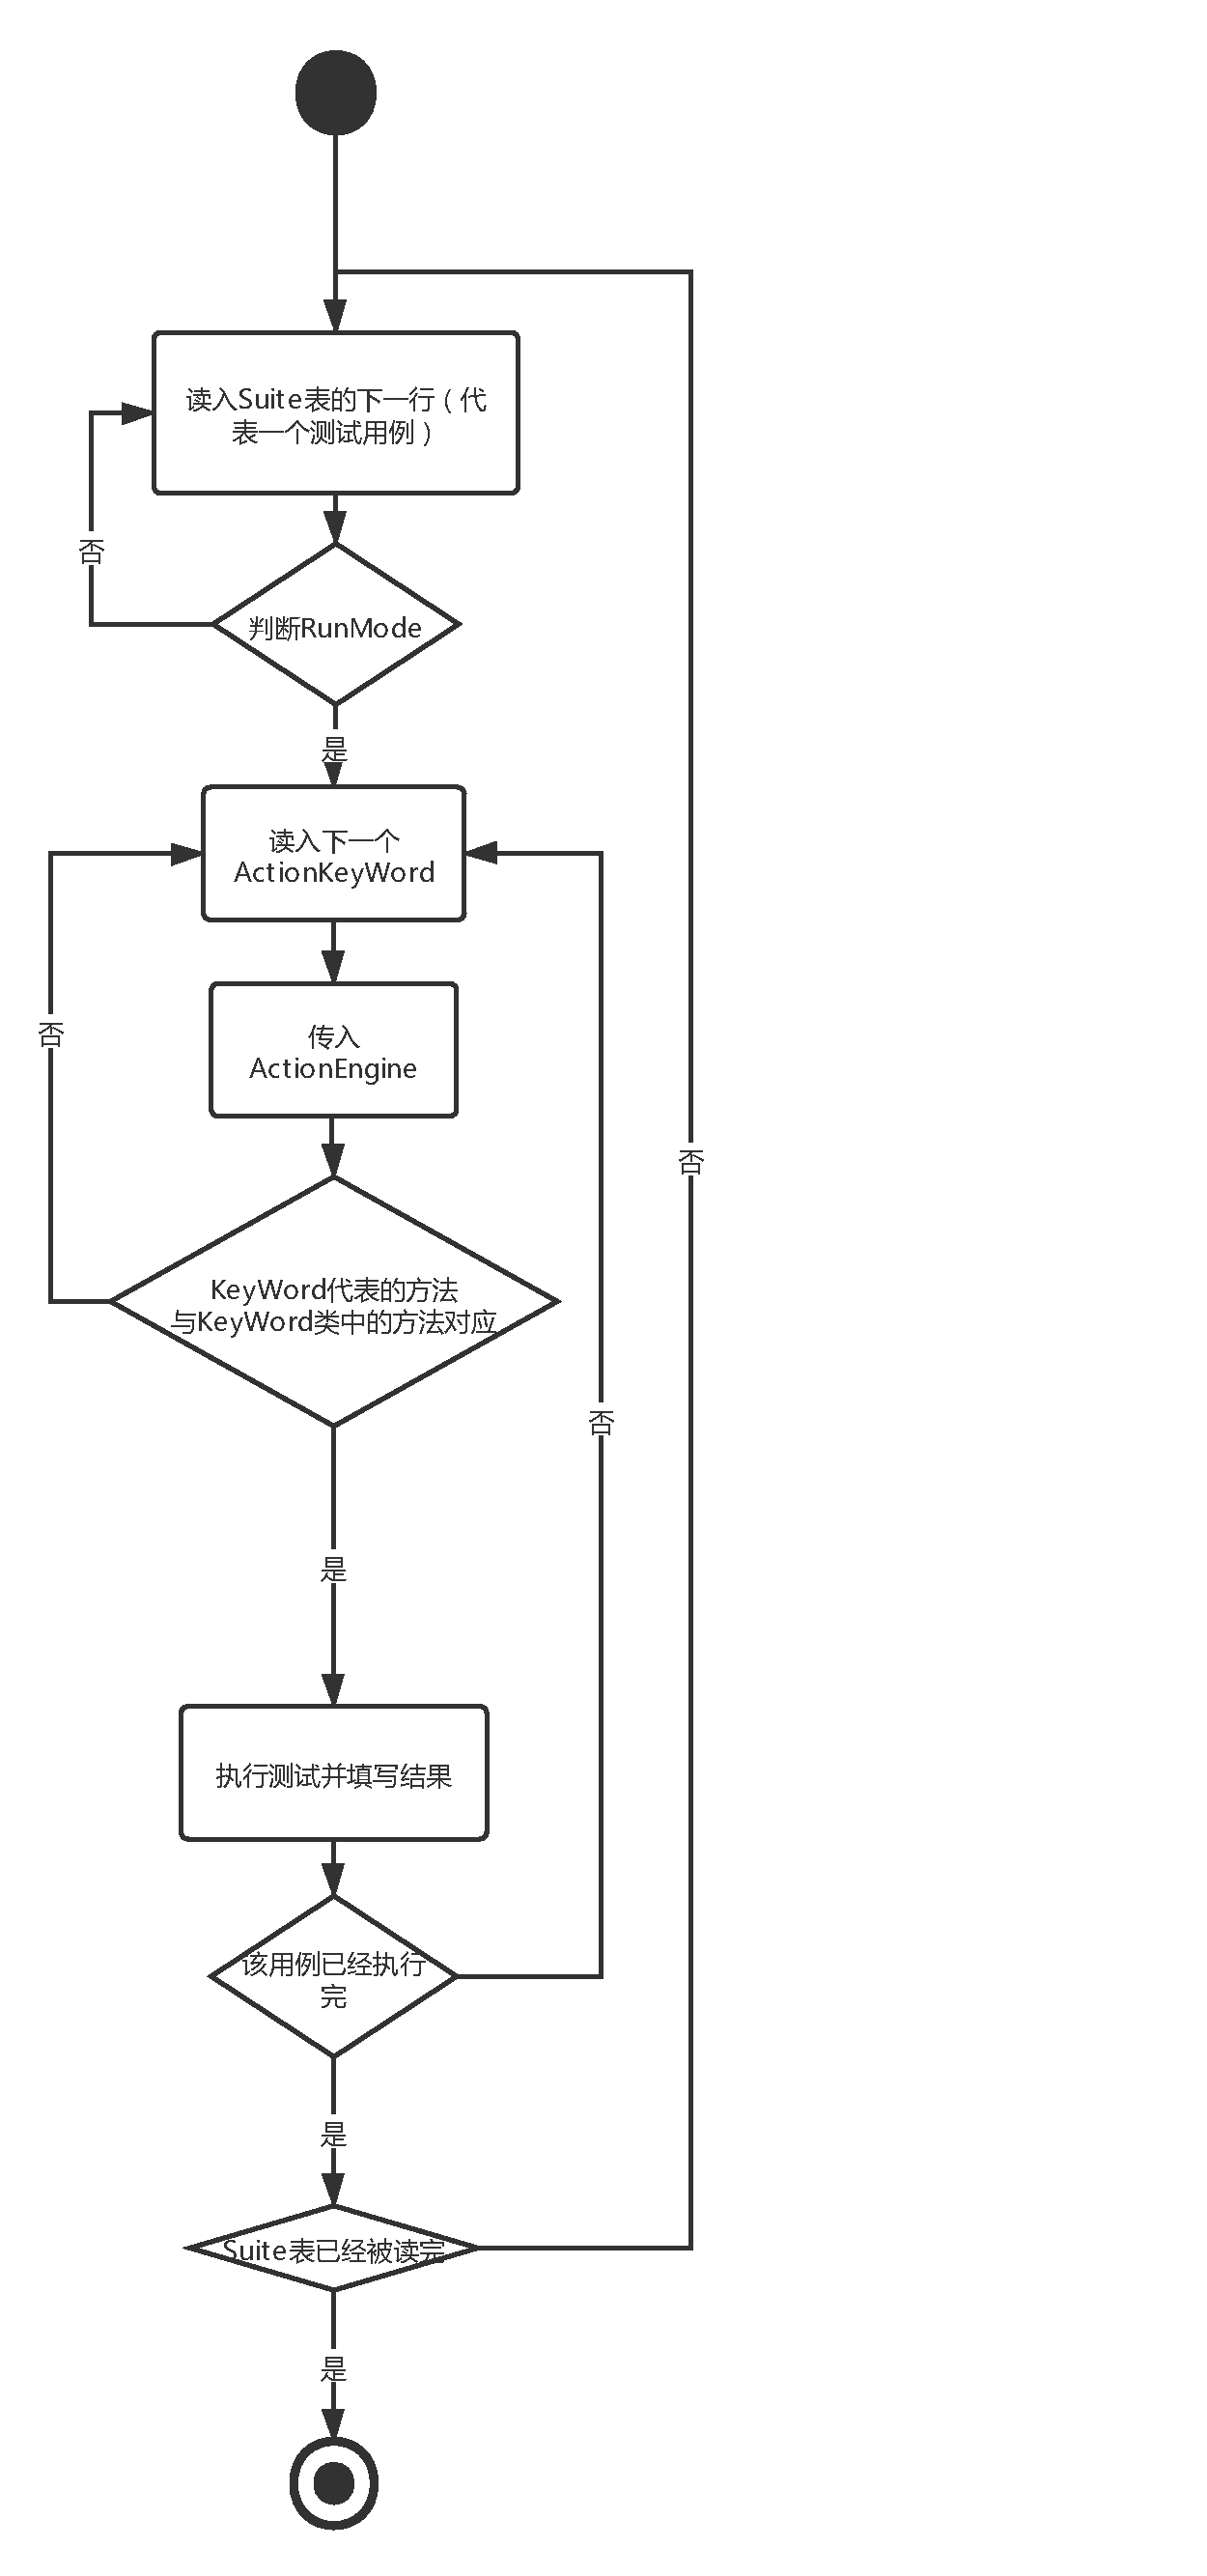
\includegraphics[scale=0.5]{./FlowChart.pdf}
  \caption{黑盒测试流程图}\label{1}
\end{figure}

\pagebreak

\hypertarget{ux9ed1ux76d2ux6d4bux8bd5ux6846ux67b6ux56feux8bf4ux660e}{%
\subsection{黑盒测试框架图说明}\label{ux9ed1ux76d2ux6d4bux8bd5ux6846ux67b6ux56feux8bf4ux660e}}

本小节内容对本小组所做的黑盒测试框架进行说明,同时也是对上一小节中的框架图的进一步说明。

\emph{框架主体结构有config,script,util三部分。}

\texttt{config}部分中的类(\texttt{LoginActionKeyWords},\texttt{AddQuestionKeyWords},它们都继承具有通用方法(如开始,结束,寻找页面元素)的\texttt{BasicKeyWords})是测试场景的关键字汇总,需要测试的测试用例都能够拆分为类中的关键字,通过关键字的组合来实现测试用例的执行。

\texttt{script}部分是测试脚本的执行入口,通过调用\texttt{Engine}类来开始测试。

\texttt{util}部分包含工具类和\texttt{Engine}类。工具类为读入Excel文件的\texttt{ExcelUtils},记录需要使用的常量(如数据文件路径,记录测试用例的表名称等)的\texttt{Constants},以及\texttt{StartEngine}和\texttt{ActionEngine}。

\texttt{StartEngine}的入口方法以代表场景的\texttt{KeyWord}类的实例作为参数,循环读取\texttt{suitSheet}里面的值,找出运行的场景,找到运行场景后根据\texttt{stepTestSuiteId}在\texttt{caseSheet}中循环查找相对应的执行步骤。

对于\texttt{caseSheet}(也即一个测试用例)的具体某行(也即场景中的某个关键字),则调用\texttt{ActionEngine}来执行,\texttt{ActionEngine}检查该行的关键字是否对应关键字类中的一个方法,如果是则调用该方法并传入可能有的参数,进行代表该关键字的步骤的执行。

\hypertarget{ux5173ux952eux5b57ux53caux6d4bux8bd5ux6570ux636eux8bbeux8ba1}{%
\section{关键字及测试数据设计}\label{ux5173ux952eux5b57ux53caux6d4bux8bd5ux6570ux636eux8bbeux8ba1}}

\hypertarget{ux6d4bux8bd5ux5173ux952eux5b57}{%
\subsection{测试关键字}\label{ux6d4bux8bd5ux5173ux952eux5b57}}

\hypertarget{ux767bux5f55}{%
\subsubsection{登录}\label{ux767bux5f55}}

登录功能需要完成用户登录出题系统的功能。登录包括打开浏览器、导航到登录网页、输入用户名、输入密码、点击认证、选择项目、登录、登出、退出。于是我们针对上述的关键步骤设计了以下关键字:

\begin{itemize}
\tightlist
\item
  openBrowser 打开浏览器
\item
  navigate 页面导航
\item
  inputName 输入用户名
\item
  inputPassword 输入密码
\item
  authButton 点击认证
\item
  chooseProject 选择项目
\item
  loginButton 登录
\item
  logoutButton 登出
\item
  quit 退出
\end{itemize}

\hypertarget{ux521bux5efaux8003ux9898}{%
\subsubsection{创建考题}\label{ux521bux5efaux8003ux9898}}

创建考题需要完成考题的相关设定。这些设定包括选择章节、选择知识点、设置作者、设置评审
、设置质管、设置类型、设置语言、设置出题日期、设置评审日期。而创建考题作为一个独立的UI测试,登录是一个基础环节。于是我们针对上述的关键步骤设计了以下关键字:

\begin{itemize}
\tightlist
\item
  loginActions 登录系统
\item
  navigateToAddQuestion 页面导航
\item
  showEditQuestion 选择添加考题
\item
  chooseChapter 选择章节
\item
  chooseKnowledgePoint 选择知识点
\item
  chooseAuthor 设置作者
\item
  chooseReviewer 设置评审
\item
  chooseQA 设置质管
\item
  chooseType 设置题目类型
\item
  startDate 设置出题开始日期
\item
  finishDate 设置出题结束日期
\item
  reviewStartDate 设置评审开始日期
\item
  reviewFinishDate 设置评审结束日期
\item
  chooseLanguage 选择语言
\item
  saveQuestion 保存考题
\end{itemize}

其中我们没有将登录拆分为更加细致的行为,这是因为登录对于创建考题环节而言是比较基础和简单的。它不是创建考题黑盒测试的考察内容。

\hypertarget{ux6d4bux8bd5ux6570ux636e}{%
\subsection{测试数据}\label{ux6d4bux8bd5ux6570ux636e}}

\hypertarget{ux767bux5f55-1}{%
\subsubsection{登录}\label{ux767bux5f55-1}}

登录的UI测试分为两个阶段,一个是用户名密码认证。如果认证成功可以进行项目选择登录。

\hypertarget{ux7b49ux4ef7ux7c7bux5212ux5206}{%
\paragraph{等价类划分}\label{ux7b49ux4ef7ux7c7bux5212ux5206}}

按输入分析等价类

\begin{table}[!htbp]
  \caption{等价类划分-输入}
  \label{Tab:bookRWCal}
  \centering
  \begin{tabular}{|p{2.0cm}|p{4.5cm}|p{6.5cm}|}
  \hline
  \textbf{输入参数} &\textbf{有效等价类} &\textbf{无效等价类} \\
  \hline
  username    & [1]已注册的用户名,且用户名下有项目,用户是enabled状态 &  [2]已注册的用户名,用户名下无项目,用户是enabled状态 \newline[3]用户名为空或null   \newline[4]未注册的非null非空的用户名  \newline[5]已注册的用户名,但是用户被禁用了 \\
  \hline
 password    & [6]用户设置的密码,与用户名相对应               & [7]用户名正确,但密码错误    \newline[8]用户名未注册    \\
  \hline
 project\_id    &  [9]项目已存在,且用户参与                    & ~                                                                                          \\
  \hline
  \end{tabular}
\end{table}

按输出分析等价类(先认证,认证成功会输出项目列表)

\begin{table}[!htbp]
  \caption{等价类划分-输出}
  \label{Tab:bookRWCal}
  \centering
  \begin{tabular}{|p{2.0cm}|p{5.5cm}|p{6.5cm}|}
  \hline
  \textbf{输入参数} &\textbf{有效等价类} &\textbf{无效等价类} \\
  \hline
  project\_list    & [10] 项目列表正确(符合要求)    &  [11] 项目列表错误(增漏或不符合要求) \\                                                                       
  \hline
  \end{tabular}
\end{table}

从字符串本身分析

\begin{table}[!htbp]
  \caption{等价类划分-字符串本身}
  \label{Tab:bookRWCal}
  \centering
  \begin{tabular}{|p{4.0cm}|p{5.5cm}|p{2.5cm}|}
  \hline
  \textbf{输入参数} &\textbf{有效等价类} &\textbf{无效等价类} \\
  \hline
  大小写    & [12]字符串全小写\newline [13]字符串全大写\newline  [14]字符串大小写混杂         & ~ \\
  \hline
  \end{tabular}
\end{table}

由于一些限制,从前端输入的时候有些情况是做不到的.比如将字符串设置为null,选择不存在的项目.

从已注册用户角色分析

\begin{table}[!htbp]
  \caption{等价类划分-角色}
  \label{Tab:bookRWCal}
  \centering
  \begin{tabular}{|p{2.0cm}|p{5.5cm}|p{6.5cm}|}
  \hline
  \textbf{输入参数} &\textbf{有效等价类} &\textbf{无效等价类} \\
  \hline
  是否为管理员    & [15]管理员 \newline [16]非管理员     & ~ \\
  \hline
    选择项目中用户的角色    &  [17]主持人\newline  [18]主持人以外的参与者    & ~ \\
  \hline
  \end{tabular}
\end{table}

边界值分析适用于具有连续取值的参数分析,登录输入没有连续取值所以不存在边界值分析。

\begin{table}[!htbp]
  \caption{等价类划分测试数据}
  \label{Tab:bookRWCal}
  \centering
  \begin{tabular}{|p{0.2cm}|p{2.0cm}|p{2.0cm}|p{1.0cm}|p{0.2cm}|p{3.0cm}|p{3.0cm}|}
  \hline
  \textbf{ID} &\textbf{覆盖的类} &\textbf{username} &\textbf{pwd} &\textbf{pj} &\textbf{Expect output} &\textbf{描述} \\
  \hline
  1  & [1][6][9][10]\newline[12][15][17] & testadmin & test &3 &  List:{test0316 test0316b 项目测试 测试登陆专用项目} 成功登陆 & 主持人成功登陆项目 \\
  \hline
 2   &[1][6][9][10]\newline[12][16][18]& jmeter004    & 123456      &  1    & list:{test0316}成功登陆     & 非主持人成功登陆项目   \\
  \hline
3 & [1][6][9][10]\newline[12][13][15][17] & TESTADMIN & test& 1& List:{test0316 test0316b 项目测试 测试登陆专用项目} 成功登陆  & 检查用户名是否大小写敏感 \\
  \hline
4   & [1][6][9][10]\newline[12][14][15][17]   & TeSTADmIN   & test  & 1& List:{test0316 test0316b 项目测试 测试登陆专用项目}成功登陆 &检查用户名是否大小写敏感 \\
  \hline
5   &[1][6][11][12]\newline[13][15][17]    & testadmin       & TEST           & ~          & 登陆失败,用户名或密码错误! & 检查用户密码是否大小写敏感 \\
  \hline
 6   & [1][6][11][13]\newline[14][15][17]    & testadmin       & teSt           &~   & 登陆失败,用户名或密码错误!        & 检查用户密码是否大小写敏感 \\
  \hline
  7   & [2][6][11][12]\newline[16]   & jmeter005   &123456     &~  & 您暂时没有分配到任何项目,或者您参与的项目已经结束.如需帮助请联系管理员! & 没有参与项目的人无法登陆 \\
  \hline
   8   &[3][8]     &~        &~         &~  & 请输入用户名和密码! & 不输入用户名和密码无法登陆         \\
  \hline
   9    &[4][8][12] & imnsb & 123456 &~ &   登陆失败,用户名或密码错误! & 未注册用户无法登陆 \\
  \hline
   10    &[5][6][14][16]   & testLogin & 123456 & ~ & 账户已被锁定,如需帮助请联系管理员!& 禁用用户无法登陆 \\
  \hline
   11    &[2][7][12][16]   & jmeter004 &~ & ~ & 请输入用户名和密码! & 密码错误且密码为空 \\
  \hline
   12    & [2][7][12][14]\newline[16] & jmeter004 & Test &~ & 登陆失败,用户名或密码错误!& 密码错误且密码不为空 \\
  \hline
  \end{tabular}
\end{table}

\hypertarget{ux521bux5efaux8003ux9898-1}{%
\subsubsection{创建考题}\label{ux521bux5efaux8003ux9898-1}}

\hypertarget{ux7b49ux4ef7ux7c7bux5212ux5206-1}{%
\paragraph{等价类划分}\label{ux7b49ux4ef7ux7c7bux5212ux5206-1}}

创建考题的UI测试具备多个输入参数,并且这些参数的取值也多种多样。我们对输入参数进行等价类划分:

\begin{table}[!htbp]
  \caption{等价类划分}
  \label{Tab:bookRWCal}
  \centering
  \begin{tabular}{|p{3.5cm}|p{5.0cm}|p{4.0cm}|}
  \hline
  \textbf{输入参数} &\textbf{有效等价类果} &\textbf{无效等价类 }\\
  \hline
  Chapter     & [1]任何章节     & [2]为空 \\
  \hline
  Knowledge point  & [3]章节下任意知识点    & [4]为空  \\
  \hline
  Author   & [5]任意用户    & [6]为空 \\
  \hline
  Reviewer    & [7]除author外用户       & [8]author \newline [9]为空 \\
  \hline
  QA     & [10]除author,reviewer外用户      & [11]author或reviewer
\newline [12]为空 \\
  \hline
  Type     & [13]任意类型       & [14]为空  \\
  \hline
  Start date   & [15]任意日期       & 16]为空  \\
  \hline
  Finish date      & [17]在开始日期及之后的日期    & [18]为空 \\
  \hline
  Review start date    & [19]出题开始日期及之后日期        & [20]为空 \newline [21]出题开始日期之前 \\
  \hline
  Review finish date   & [22]评审开始日期及之后的日期,且不早于出题结束日期    & [23]为空 \newline  [24]出题结束日期之前 \\
  \hline
  Language    & [25]任意语言    & [26]为空 \\
  \hline
  \end{tabular}
\end{table}

表2是根据等价类划分设计的测试用例,其中c0表示第一个章节,k0表示该章节第一个知识点,u0表示成员1,u1表示成员2,u2表示成员3,t0表示类型为情景题,l0表示语言为中文。

\begin{table}[!htbp]
  \caption{等价类划分测试数据}
  \centering
  \begin{tabular}{|p{0.35cm}|p{1.2cm}|p{0.22cm}|p{0.22cm}|p{0.22cm}|p{0.22cm}|p{0.22cm}|p{0.22cm}|p{0.9cm}|p{0.9cm}|p{0.9cm}|p{0.9cm}|p{0.22cm}|p{0.8cm}|}
  \hline
  \textbf{ID} & \textbf{类} & \multicolumn{11}{c|}{\textbf{输入参数}} & \textbf{预期}  \\ 
  \hline
1   & 1,3,5,7, 10,13,15, 17,19,22, 25 & c0  & k0 & u0 & u1 & u2 & t0  & 2020-05-03 & 2020-05-03 & 2020-05-03 & 2020-05-03 & l0 & 成功   \\
  \hline
2   & 2  & 空 & k0  & u0 & u1 & u2 & t0  & 2020-05-03 & 2020-05-03  
& 2020-05-03 & 2020-05-03 & l0 & 失败   \\
  \hline
3   & 4  & c0 & 空 & u0 & u1 & u2 & t0  & 2020-05-03 & 2020-05-04  
& 2020-05-03 & 2020-05-04 & l0 & 失败   \\
  \hline
4   & 6  & c0 & k0  & 空 & u1 & u2 & t0  & 2020-05-03 & 2020-05-04  
& 2020-05-03 & 2020-05-04 & l0 & 失败   \\
  \hline
5   & 8  & c0 & k0  & u0 & u0 & u2 & t0  & 2020-05-03 & 2020-05-04  
& 2020-05-03 & 2020-05-04 & l0 & 失败   \\
  \hline
6   & 9  & c0 & k0  & u0 & 空 & u2 & t0  & 2020-05-03 & 2020-05-04  
& 2020-05-03 & 2020-05-04 & l0 & 失败   \\
  \hline
7   & 11 & c0 & k0  & u0 & u1 & u1 & t0  & 2020-05-03 & 2020-05-04  
& 2020-05-03 & 2020-05-04 & 0  & 失败   \\
  \hline
8   & 12 & c0 & k0  & u0 & u1 & 空 & t0  & 2020-05-03 & 2020-05-04  
& 2020-05-03 & 2020-05-04 & l0 & 失败   \\
  \hline
9   & 14 & c0 & k0  & u0 & u1 & u2 & 空  & 2020-05-03 & 2020-05-04  
& 2020-05-03 & 2020-05-04 & l0 & 失败   \\
  \hline 
10  & 16 & c0 & k0  & u0 & u1 & u2 & t0  & 空         & 2020-05-04  
& 2020-05-03 & 2020-05-04 & l0 & 失败   \\
  \hline
11  & 18 & c0 & k0  & u0 & u1 & u2 & t0  & 2020-05-03 & 空  
& 2020-05-03 & 2020-05-04 & l0 & 失败   \\
  \hline
12  & 20 & c0 & k0  & u0 & u1 & u2 & t0  & 2020-05-03 & 2020-05-04  
& 空         & 2020-05-04 & l0 & 失败   \\
  \hline
13  & 21 & c0 & k0  & u0 & u1 & u2 & t0  & 2020-05-03 & 2020-05-04  
& 2020-04-30 & 2020-05-04 & l0 & 失败   \\
  \hline
14  & 23 & c0 & k0  & u0 & u1 & u2 & t0  & 2020-05-03 & 2020-05-04  
& 2020-05-03 & 空         & l0 & 失败   \\
  \hline
15  & 24 & c0 & k0  & u0 & u1 & u2 & t0  & 2020-05-03 & 2020-05-04  
& 2020-05-03 & 2020-05-03 & l0 & 失败   \\
  \hline
16  & 26 & 0  & 0  & u0 & u1 & u2 & t0  & 2020-05-03 & 2020-05-04  
& 2020-05-03 & 2020-05-04 & 空 & 失败   \\

  \hline
  \end{tabular}
\end{table}

\hypertarget{ux8fb9ux754cux503cux5206ux6790}{%
\paragraph{边界值分析}\label{ux8fb9ux754cux503cux5206ux6790}}

边界值分析适用于具有连续取值的参数分析,题目中具有连续取值的只有出题日期与评审日期。
其中出题开始日期不存在边界限定,故不考虑。而对于评审结束日期,它的边界值与评审开始日期和出题结束日期相关。由于这两个日期不存在约束关系,
故它的多个边界值条件可以同时成立。对于不存在连续取值的参数,此处边界值分析不再进行罗列,在测试数据中会使用固定的取值。

\begin{table}[!htbp]
  \caption{边界值分析}
  \label{Tab:bookRWCal}
  \centering
  \begin{tabular}{|p{6.0cm}|p{6.5cm}|}
  \hline
  \textbf{输入参数} &\textbf{边界值} \\
  \hline
  Finish date     & [27]与start date相同   \newline [28] start date后一天 \\
  \hline
  Review start date     & [29]Start date前一天     \newline [30]与Start date相同  \newline  [31]Start date后一天 \\
  \hline
  Review finish date     & [32]与Review start date相同     \newline [33]Review start date后一天 \newline [34]Finish date前一天 \newline [35]与Finish date相同  \newline  [36]Finish date后一天\\
  \hline
  \end{tabular}
\end{table}

表4是根据边界值分析设计的测试数据。

\begin{table}[!htbp]
  \caption{边界值分析测试数据}
  \centering
  \begin{tabular}{|p{0.35cm}|p{1.2cm}|p{0.22cm}|p{0.22cm}|p{0.22cm}|p{0.22cm}|p{0.22cm}|p{0.22cm}|p{0.9cm}|p{0.9cm}|p{0.9cm}|p{0.9cm}|p{0.22cm}|p{0.8cm}|}
  \hline
  \textbf{ID} & \textbf{类} & \multicolumn{11}{c|}{\textbf{输入参数}} & \textbf{预期}  \\ 
  \hline
17   & 27,30, 32,35 & c0  & k0  & u0 & u1 & u2 & t0  & 2020-05-03 & 2020-05-03 & 2020-05-03 & 2020-05-03 & l0 & 成功   \\
  \hline
18   & 28,31, 33,36 & c0  & k0  & u0 & u1 & u2 & t0  & 2020-05-03 & 2020-05-04 & 2020-05-04 & 2020-05-05 & l0 & 成功   \\
  \hline
19   & 29           & c0  & k0  & u0 & u1 & u2 & t0  & 2020-05-03 & 2020-05-04 & 2020-05-02 & 2020-05-04 & l0 & 失败   \\
  \hline
20   & 34           & c0  & k0  & u0 & u1 & u2 & t0  & 2020-05-03 & 2020-05-04 & 2020-05-03 & 2020-05-03 & l0 & 失败   \\
  \hline
  \end{tabular}
\end{table}

\pagebreak

\hypertarget{ux6d4bux8bd5ux811aux672cux5b9eux73b0ux53caux8fd0ux884c}{%
\section{测试脚本实现及运行}\label{ux6d4bux8bd5ux811aux672cux5b9eux73b0ux53caux8fd0ux884c}}

\hypertarget{ux811aux672cux5b9eux73b0ux65b9ux5f0f}{%
\subsection{脚本实现方式}\label{ux811aux672cux5b9eux73b0ux65b9ux5f0f}}

脚本的实现主要参照https://my.oschina.net/hellotest/blog/531932
中,通过java反射机制,使用poi包操作excel关键字表,使用selenium的jar包进行自动化录制测试操作,以完成自动化测试框架。

\hypertarget{ux51faux9898ux6d4bux8bd5ux811aux672cux5b9eux73b0}{%
\subsubsection{出题测试脚本实现}\label{ux51faux9898ux6d4bux8bd5ux811aux672cux5b9eux73b0}}

\hypertarget{ux6267ux884cux6d41ux7a0b}{%
\paragraph{执行流程}\label{ux6267ux884cux6d41ux7a0b}}

\begin{itemize}
\tightlist
\item
  登陆
\item
  导航到添加题目
\item
  显示添加题目对话框
\item
  选择章节
\item
  选择知识点
\item
  选择作者
\item
  选择审核者
\item
  选择质量审核
\item
  选择种类
\item
  填写开始日期
\item
  填写结束日期
\item
  填写审核开始日期
\item
  填写审核结束日期
\item
  选择语言
\item
  保存问题
\end{itemize}

\hypertarget{ux8fd0ux884cux622aux56feux53caux8bf4ux660e}{%
\subsection{运行截图及说明}\label{ux8fd0ux884cux622aux56feux53caux8bf4ux660e}}

\hypertarget{ux63a7ux5236ux53f0ux622aux56fe}{%
\subsubsection{控制台截图}\label{ux63a7ux5236ux53f0ux622aux56fe}}

\begin{figure}
  \centering
  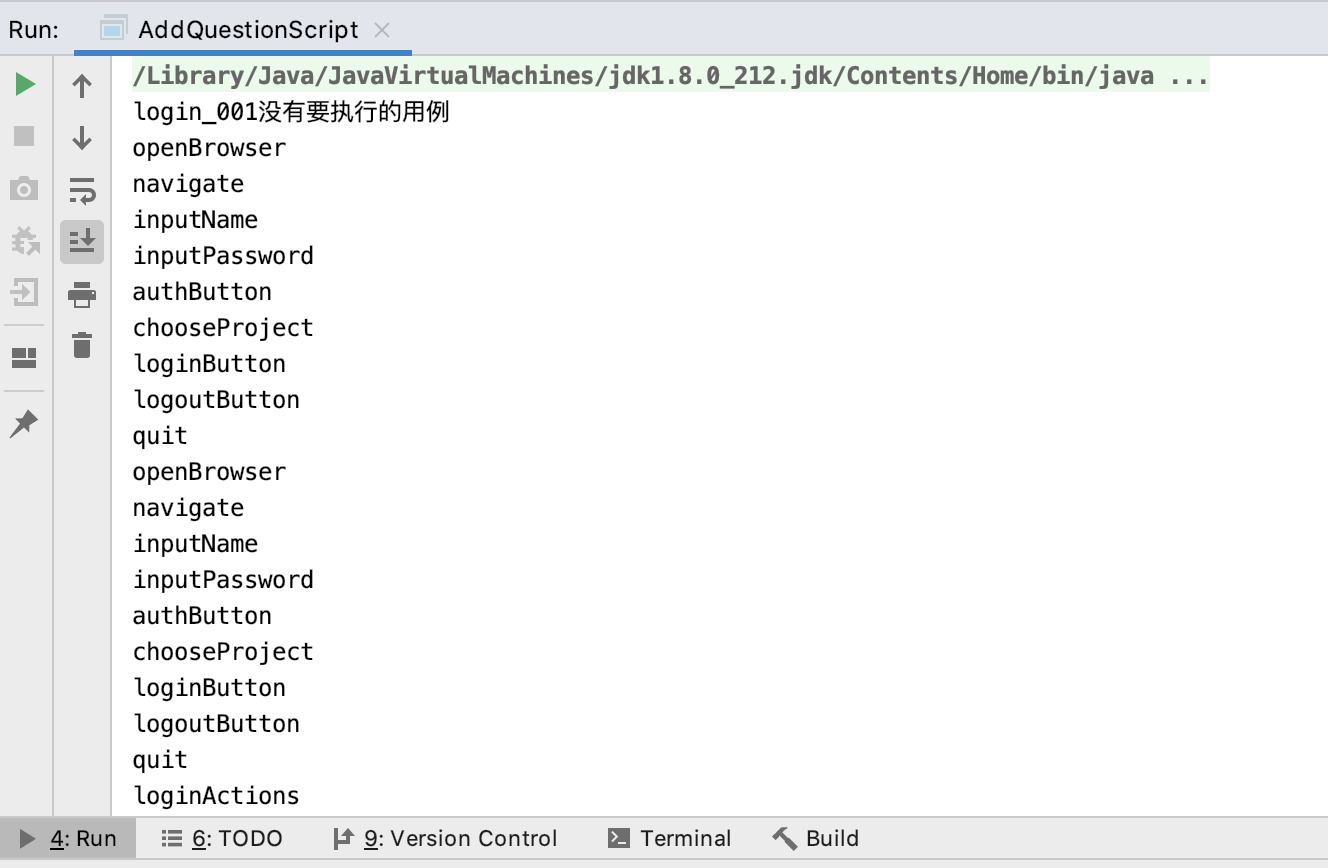
\includegraphics[scale=0.33]{./screenshots/console.jpg}
  \caption{console screenshot}\label{4}
\end{figure}

\hypertarget{ux8fd0ux884cux8bf4ux660e}{%
\subsubsection{运行说明}\label{ux8fd0ux884cux8bf4ux660e}}

\hypertarget{ux6d4bux8bd5ux7528ux4f8bux8fd0ux884cux8fc7ux7a0bux8bb0ux5f55}{%
\subsection{测试用例运行过程记录}\label{ux6d4bux8bd5ux7528ux4f8bux8fd0ux884cux8fc7ux7a0bux8bb0ux5f55}}

本小组对本次黑盒测试的过程进行了记录,这些记录的内容完整地展现了本小组的黑盒测试用例设计以及测试环境、测试流程。测试过程视频可以通过如下方式进行查看,各平台的内容一致:

\begin{itemize}
\tightlist
\item
  优酷视频(访问密码为FudanUniversitySoftwareSchool):\url{https://v.youku.com/v_show/id_XNDY2NzE4NzQxMg==.html}
\item
  搜狐视频(访问密码为FudanUniversitySoftwareSchool):\url{https://tv.sohu.com/v/dXMvMTI2MDUwODM0LzE5MzY2NDI2OS5zaHRtbA==.html}
\item
  百度网盘(提取码为ut6f):\url{https://pan.baidu.com/s/1FI7FPEp3_piM6QpkU1B7WQ}
\end{itemize}

\pagebreak

\hypertarget{ux53c2ux8003ux6587ux732e}{%
\section*{参考文献}\label{ux53c2ux8003ux6587ux732e}}
\addcontentsline{toc}{section}{参考文献}

\hypertarget{refs}{}
\leavevmode\hypertarget{ref-innovativeInternationalisation}{}%
International Organization for Standardization. 2014. \emph{Systems and
Software Engineering --- Systems and Software Quality Requirements and
Evaluation (SQuaRE) --- Guide to SQuaRE}. \emph{International
Organization for Standardization}. Vol. 2014.
\url{https://www.iso.org/standard/64764.html}.

\leavevmode\hypertarget{ref-innovative1}{}%
中国国家标准化管理委员会. 2016. \emph{GB/T
25000.51-2016《系统与软件工程系统与软件质量要求和评价 (SQuaRE) 第 51
部分 : 就绪可用软件产品 (RUSP) 的质量要求和测试细则》}.
\emph{系统与软件工程系统与软件质量要求和评价 (SQuaRE)}. Vol. 51.
中国国家标准化管理委员会. \url{http://openstd.samr.gov.cn}.

\leavevmode\hypertarget{ref-innovative3}{}%
---------. 2017a. \emph{GB/T 25000.12-2017《系统与软件工程
系统与软件质量要求和评价(SQuaRE) 第12部分:数据质量模型》}.
\emph{系统与软件工程系统与软件质量要求和评价 (SQuaRE)}. Vol. 12.
中国国家标准化管理委员会. \url{http://openstd.samr.gov.cn}.

\leavevmode\hypertarget{ref-innovative4}{}%
---------. 2017b. \emph{GB/T 25000.24-2017《系统与软件工程
系统与软件质量要求和评价(SQuaRE) 第24部分:数据质量测量》}.
\emph{系统与软件工程系统与软件质量要求和评价 (SQuaRE)}. Vol. 24.
中国国家标准化管理委员会. \url{http://openstd.samr.gov.cn}.

\leavevmode\hypertarget{ref-innovative5}{}%
---------. 2018. \emph{GB/T 25000.40-201《系统与软件工程
系统与软件质量要求和评价(SQuaRE) 第40部分:评价过程》}.
\emph{系统与软件工程系统与软件质量要求和评价 (SQuaRE)}. Vol. 40.
中国国家标准化管理委员会. \url{http://openstd.samr.gov.cn}.

\leavevmode\hypertarget{ref-innovative2}{}%
---------. 2019. \emph{GB/T 25000.23-2019《系统与软件工程
系统与软件质量要求和评价(SQuaRE) 第23部分:系统与软件产品质量测量》}.
\emph{系统与软件工程系统与软件质量要求和评价 (SQuaRE)}. Vol. 23.
中国国家标准化管理委员会. \url{http://openstd.samr.gov.cn}.

\end{document}
